% HIEU Model Architecture Diagram - Detailed Clean Version
\documentclass[tikz,border=15pt]{standalone}
\usepackage{tikz}
\usetikzlibrary{shapes.geometric, arrows.meta, positioning, fit, backgrounds, calc, decorations.pathreplacing}
\usepackage{amsmath}
\usepackage{amssymb}

% Define colors
\definecolor{inputcolor}{RGB}{227, 242, 253}
\definecolor{regimecolor}{RGB}{255, 205, 210}
\definecolor{graphcolor}{RGB}{200, 230, 201}
\definecolor{freqcolor}{RGB}{255, 236, 179}
\definecolor{concatcolor}{RGB}{255, 224, 178}
\definecolor{corecolor}{RGB}{179, 229, 252}
\definecolor{hypercolor}{RGB}{225, 190, 231}
\definecolor{outputcolor}{RGB}{248, 187, 208}
\definecolor{streamorange}{RGB}{255, 152, 0}
\definecolor{streamgreen}{RGB}{76, 175, 80}

\begin{document}
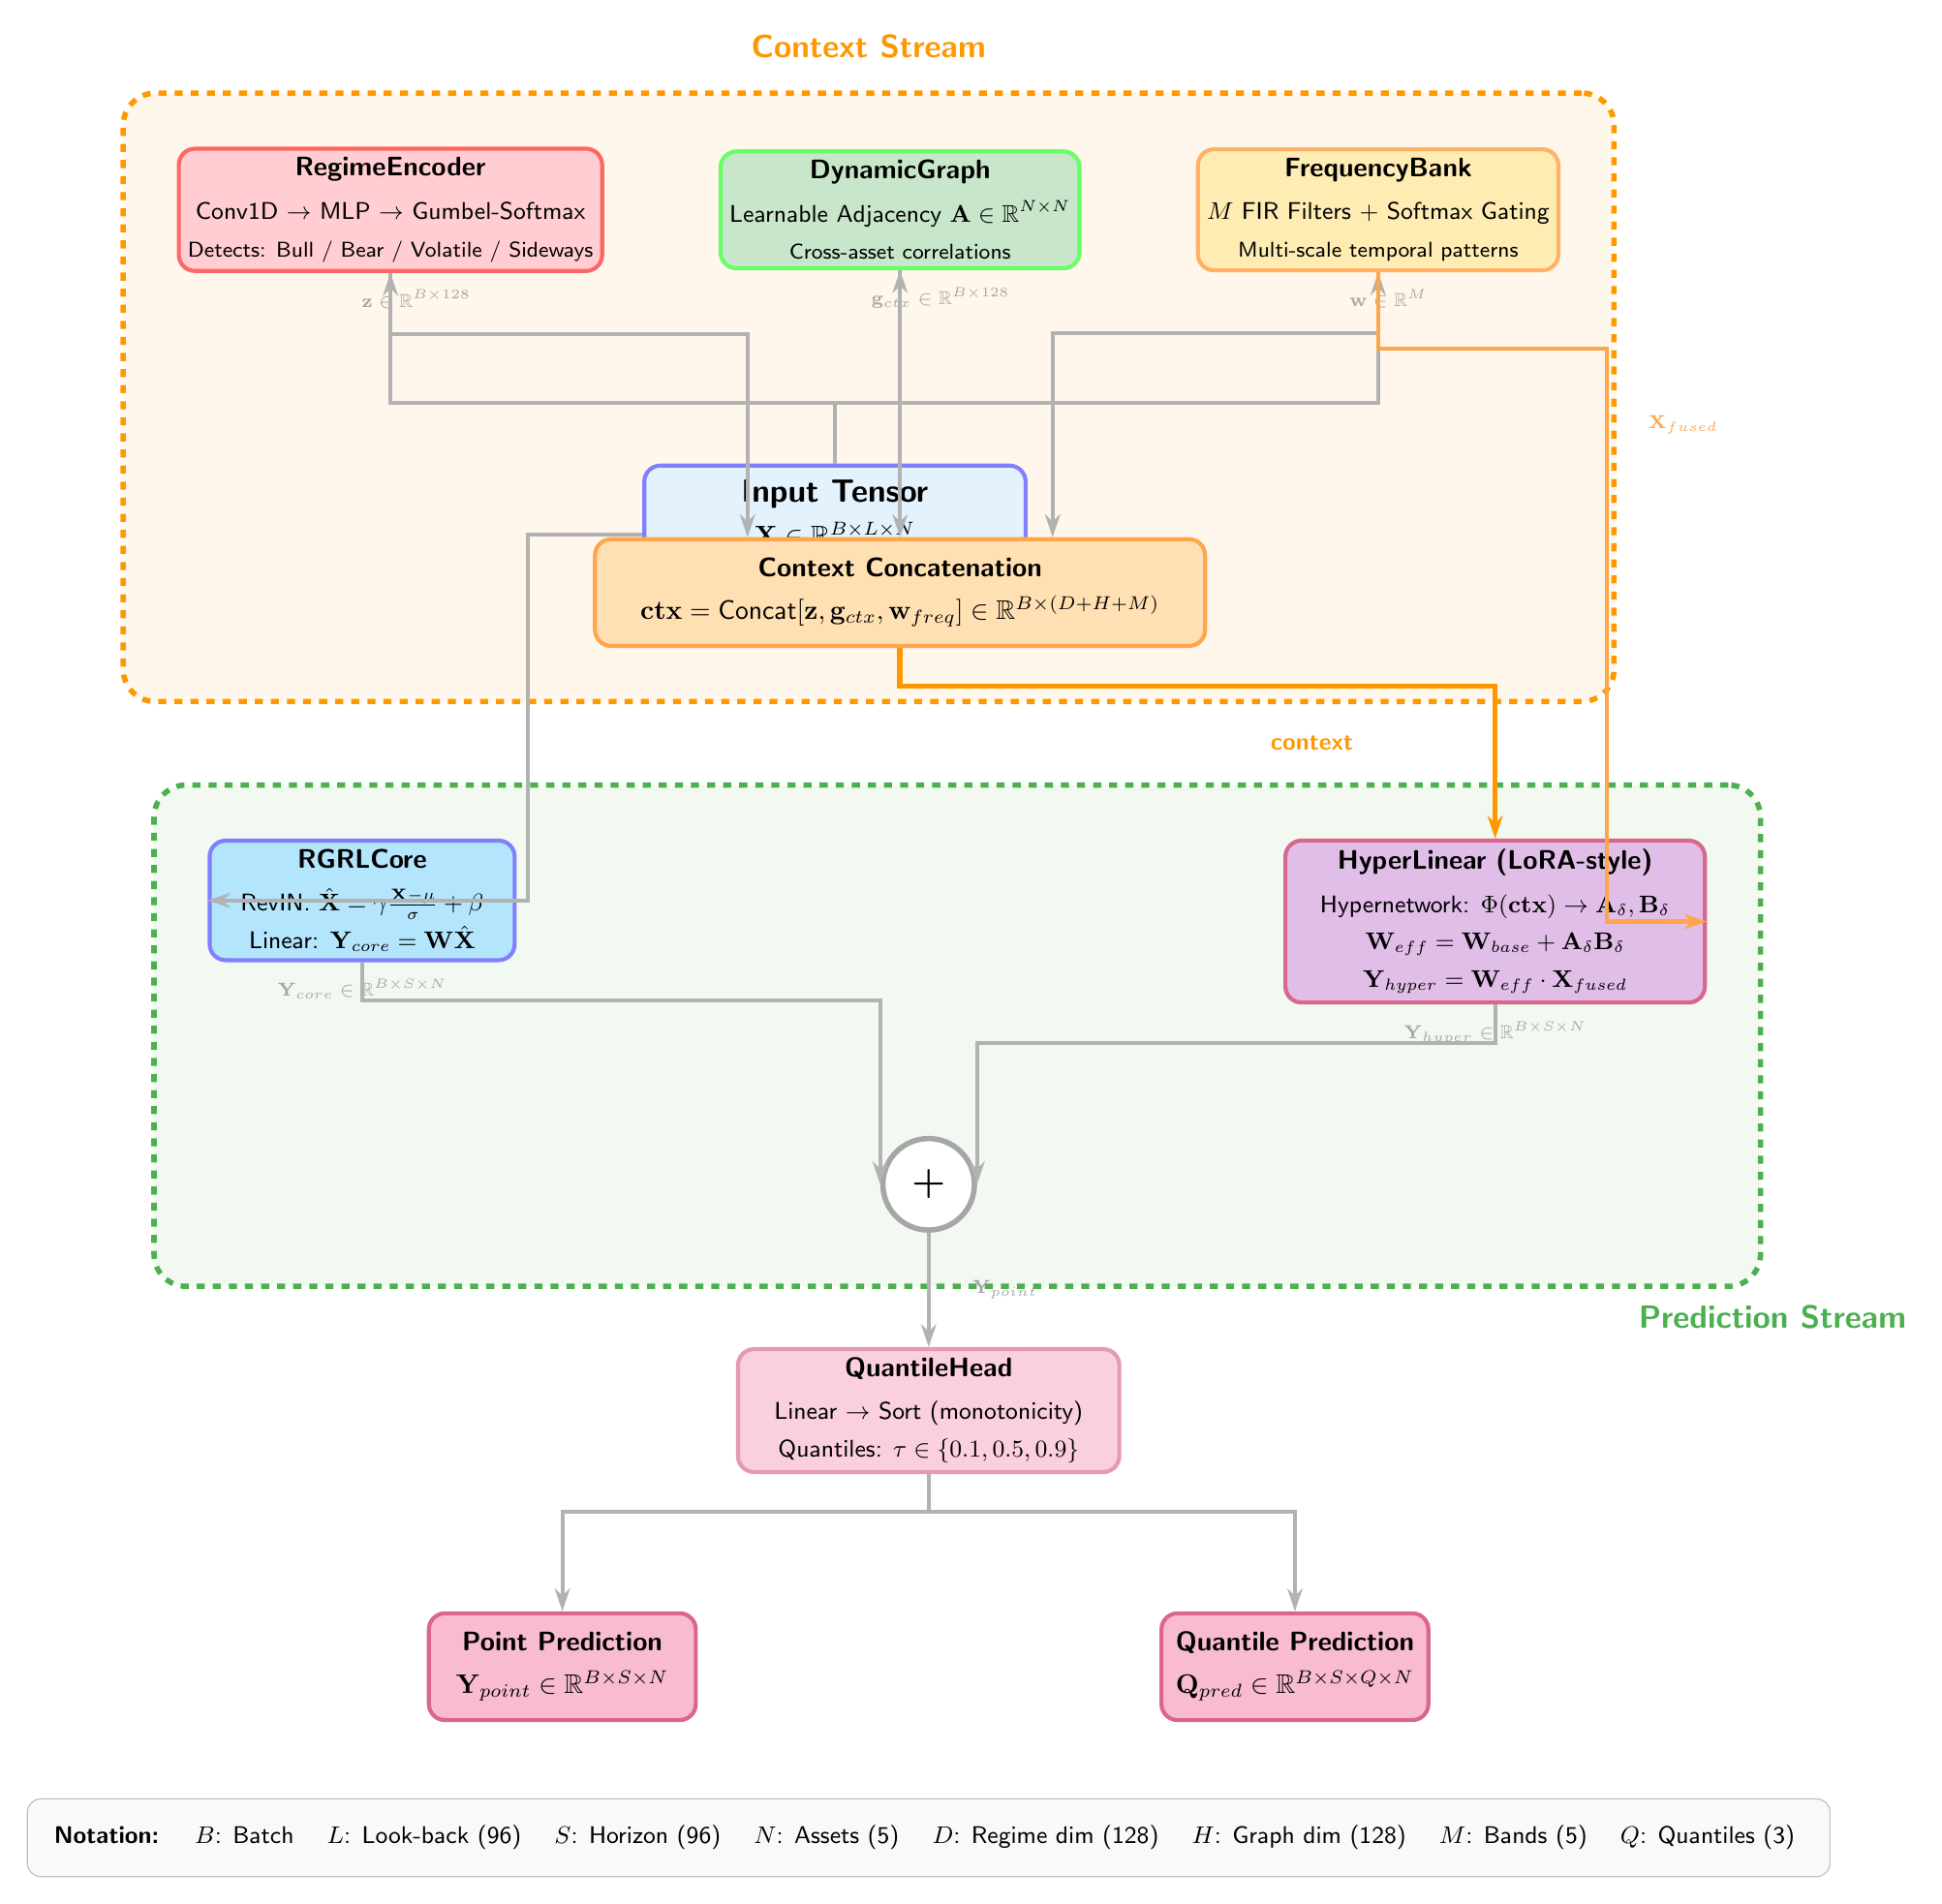
\begin{tikzpicture}[
    node distance=1.5cm,
    >={Stealth[length=3mm, width=2mm]},
    mainbox/.style={rectangle, draw, rounded corners=6pt, minimum width=4cm, minimum height=1.4cm, align=center, font=\sffamily, line width=1.5pt},
    smallbox/.style={rectangle, draw, rounded corners=4pt, minimum width=3cm, minimum height=0.8cm, align=center, font=\sffamily\small, line width=1pt},
    arrow/.style={->, line width=1.5pt, draw=gray!60},
    contextarrow/.style={->, line width=2pt, draw=streamorange},
    tensorlabel/.style={font=\sffamily\scriptsize, text=gray!70},
    scale=1
]

% ==================== INPUT ====================
\node[mainbox, fill=inputcolor, draw=blue!50, minimum width=5cm, minimum height=1.8cm] (input) {
    \textbf{\large Input Tensor}\\[4pt]
    $\mathbf{X} \in \mathbb{R}^{B \times L \times N}$\\[2pt]
    {\small (batch, sequence, assets)}
};

% ==================== CONTEXT STREAM ====================
% RegimeEncoder
\node[mainbox, fill=regimecolor, draw=red!60, above left=2.5cm and 0.5cm of input] (regime) {
    \textbf{RegimeEncoder}\\[4pt]
    {\small Conv1D $\to$ MLP $\to$ Gumbel-Softmax}\\[2pt]
    {\footnotesize Detects: Bull / Bear / Volatile / Sideways}
};
\node[tensorlabel, below right=0.1cm and -0.5cm of regime.south] {$\mathbf{z} \in \mathbb{R}^{B \times 128}$};

% DynamicGraph
\node[mainbox, fill=graphcolor, draw=green!60, right=1.5cm of regime] (graph) {
    \textbf{DynamicGraph}\\[4pt]
    {\small Learnable Adjacency $\mathbf{A} \in \mathbb{R}^{N \times N}$}\\[2pt]
    {\footnotesize Cross-asset correlations}
};
\node[tensorlabel, below right=0.1cm and -0.5cm of graph.south] {$\mathbf{g}_{ctx} \in \mathbb{R}^{B \times 128}$};

% FrequencyBank
\node[mainbox, fill=freqcolor, draw=orange!60, right=1.5cm of graph] (freq) {
    \textbf{FrequencyBank}\\[4pt]
    {\small $M$ FIR Filters + Softmax Gating}\\[2pt]
    {\footnotesize Multi-scale temporal patterns}
};
\node[tensorlabel, below right=0.1cm and -0.5cm of freq.south] {$\mathbf{w} \in \mathbb{R}^{M}$};

% Context Concatenation
\node[mainbox, fill=concatcolor, draw=orange!70, below=3.5cm of graph, minimum width=8cm] (concat) {
    \textbf{Context Concatenation}\\[4pt]
    $\mathbf{ctx} = \text{Concat}[\mathbf{z}, \mathbf{g}_{ctx}, \mathbf{w}_{freq}] \in \mathbb{R}^{B \times (D+H+M)}$
};

% ==================== PREDICTION STREAM ====================
% RGRLCore
\node[mainbox, fill=corecolor, draw=blue!50, below left=2.5cm and 1cm of concat] (core) {
    \textbf{RGRLCore}\\[4pt]
    {\small RevIN: $\hat{\mathbf{X}} = \gamma \frac{\mathbf{X}-\mu}{\sigma} + \beta$}\\[2pt]
    {\small Linear: $\mathbf{Y}_{core} = \mathbf{W}\hat{\mathbf{X}}$}
};
\node[tensorlabel, below=0.1cm of core] {$\mathbf{Y}_{core} \in \mathbb{R}^{B \times S \times N}$};

% HyperLinear
\node[mainbox, fill=hypercolor, draw=purple!60, below right=2.5cm and 1cm of concat, minimum width=5.5cm] (hyper) {
    \textbf{HyperLinear (LoRA-style)}\\[4pt]
    {\small Hypernetwork: $\Phi(\mathbf{ctx}) \to \mathbf{A}_\delta, \mathbf{B}_\delta$}\\[2pt]
    {\small $\mathbf{W}_{eff} = \mathbf{W}_{base} + \mathbf{A}_\delta \mathbf{B}_\delta$}\\[2pt]
    {\small $\mathbf{Y}_{hyper} = \mathbf{W}_{eff} \cdot \mathbf{X}_{fused}$}
};
\node[tensorlabel, below=0.1cm of hyper] {$\mathbf{Y}_{hyper} \in \mathbb{R}^{B \times S \times N}$};

% Addition
\node[circle, draw=gray!70, fill=white, line width=2pt, minimum size=1.2cm, below=2cm of $(core.south)!0.5!(hyper.south)$] (add) {\Large\textbf{+}};

% QuantileHead
\node[mainbox, fill=outputcolor!70, draw=purple!40, below=1.5cm of add, minimum width=5cm] (qhead) {
    \textbf{QuantileHead}\\[4pt]
    {\small Linear $\to$ Sort (monotonicity)}\\[2pt]
    {\small Quantiles: $\tau \in \{0.1, 0.5, 0.9\}$}
};

% Outputs
\node[mainbox, fill=outputcolor, draw=purple!60, below left=1.8cm and 0.5cm of qhead, minimum width=3.5cm] (ypoint) {
    \textbf{Point Prediction}\\[4pt]
    $\mathbf{Y}_{point} \in \mathbb{R}^{B \times S \times N}$
};

\node[mainbox, fill=outputcolor, draw=purple!60, below right=1.8cm and 0.5cm of qhead, minimum width=3.5cm] (qpred) {
    \textbf{Quantile Prediction}\\[4pt]
    $\mathbf{Q}_{pred} \in \mathbb{R}^{B \times S \times Q \times N}$
};

% ==================== ARROWS ====================
% Input to Context modules
\draw[arrow] (input.north) -- ++(0, 0.8) -| (regime.south);
\draw[arrow] (input.north) -- ++(0, 0.8) -| (graph.south);
\draw[arrow] (input.north) -- ++(0, 0.8) -| (freq.south);

% Context modules to Concat
\draw[arrow] (regime.south) -- ++(0, -0.8) -| ([xshift=-2cm]concat.north);
\draw[arrow] (graph.south) -- (concat.north);
\draw[arrow] (freq.south) -- ++(0, -0.8) -| ([xshift=2cm]concat.north);

% Input to RGRLCore (direct path)
\draw[arrow] (input.west) -- ++(-1.5, 0) |- (core.west);

% Concat to HyperLinear (context conditioning) - THICK ARROW
\draw[contextarrow] (concat.south) -- ++(0, -0.5) -| (hyper.north);
\node[font=\sffamily\small\bfseries, text=streamorange] at ($(concat.south)!0.5!(hyper.north) + (1.5, 0)$) {context};

% FrequencyBank to HyperLinear (fused input)
\draw[arrow, orange!70] (freq.south) -- ++(0, -1) -- ++(3, 0) |- (hyper.east);
\node[tensorlabel, text=orange!70] at ($(freq.south) + (4, -2)$) {$\mathbf{X}_{fused}$};

% Core and Hyper to Add
\draw[arrow] (core.south) -- ++(0, -0.5) -| (add.west);
\draw[arrow] (hyper.south) -- ++(0, -0.5) -| (add.east);

% Add to QHead
\draw[arrow] (add.south) -- (qhead.north);
\node[tensorlabel] at ($(add.south)!0.5!(qhead.north) + (1, 0)$) {$\mathbf{Y}_{point}$};

% QHead to outputs
\draw[arrow] (qhead.south) -- ++(0, -0.5) -| (ypoint.north);
\draw[arrow] (qhead.south) -- ++(0, -0.5) -| (qpred.north);

% ==================== STREAM BOXES ====================
\begin{scope}[on background layer]
    % Context Stream
    \node[rectangle, rounded corners=12pt, draw=streamorange, dashed, line width=2pt, 
          fill=streamorange!8, inner sep=20pt,
          fit=(regime)(graph)(freq)(concat)] (ctxbox) {};
    
    % Prediction Stream
    \node[rectangle, rounded corners=12pt, draw=streamgreen, dashed, line width=2pt,
          fill=streamgreen!8, inner sep=20pt,
          fit=(core)(hyper)(add)] (predbox) {};
\end{scope}

% Stream Labels
\node[font=\sffamily\large\bfseries, text=streamorange, above=0.3cm of ctxbox.north] {Context Stream};
\node[font=\sffamily\large\bfseries, text=streamgreen, below left=0.1cm and -2cm of predbox.south east] {Prediction Stream};

% ==================== NOTATION BOX ====================
\node[rectangle, draw=gray!50, rounded corners=5pt, fill=gray!5, 
      below=1cm of $(ypoint.south)!0.5!(qpred.south)$, 
      minimum width=10cm, inner sep=10pt, align=left, font=\sffamily\small] (notation) {
    \textbf{Notation:} \quad
    $B$: Batch \quad
    $L$: Look-back (96) \quad
    $S$: Horizon (96) \quad
    $N$: Assets (5) \quad
    $D$: Regime dim (128) \quad
    $H$: Graph dim (128) \quad
    $M$: Bands (5) \quad
    $Q$: Quantiles (3)
};

\end{tikzpicture}
\end{document}
